\documentclass{article}
\usepackage[utf8]{vietnam}
\usepackage{graphicx}
\usepackage{amssymb}
\usepackage{titlesec}
\usepackage{lipsum}

\graphicspath{ {./images/} }
\newcommand\tab[1][1cm]{\hspace*{#1}}

\title{NÃO BỘ NÓI GÌ VỀ BẠN}

\begin{document}
\maketitle

30-July-2024
\section{Tôi là ai?}

\tab Những suy nghĩ, ước mơ, kỉ niệm, kinh nghiệm đều xuất phát từ bộ não. Chỉ cần một sự thay đổi nhỏ (do chấn thương, ma túy) tính cách của bạn sẽ thay đổi theo tức khắc. Để hiểu rõ điều đó xảy ra như thế nào, hãy xuất phát từ điểm khởi đầu.\\
\tab Khi sinh ra, loài người chỉ là những sinh vật yếu đuối. Chúng ta mất khoảng 1 năm không thể tự đi lại, 2 năm để biểu đạt những suy nghĩ của mình, nhiều năm nữa để tự lo liệu cho bản thân. Chúng ta phụ thuộc hoàn toàn vào những người xung quanh để tồn tại. Trong khi đó các động vật có vú khác lại tự lập một cách đáng kinh ngạc sau khi chúng được sinh ra, cá heo sinh ra có thể tự bơi lội, ngựa vằn non có thể chạy trong vòng 45 phút sau sinh. Nếu chỉ nhìn bề ngoài, lợi thế lớn thuộc về các loài khác, nhưng trên thực tế nó biểu thị một giới hạn. Động vật sơ sinh phát triển nhanh chóng bởi vì não của chúng là kết nối cứng, điều này vô tình chung khiến động vật đó chỉ có thể hoạt động trong một vị trí cụ thể của hệ sinh thái. Trong khi đó, con người với kết nối mềm dẻo (chưa hoàn thiện) - sẽ được hình thành nốt bằng trải nghiệm sống, lại có khả năng phát triển mạnh mẽ trong nhiều môi trường khác nhau. Cần làm rõ một xí ở đây, bộ não con người từ khi sinh ra đã có một số lượng kết nối cứng di truyền nhất định (thở, khóc, bú, biểu cảm khuôn mặt, \dots)
\tab Có 2 yếu tố chính hình thành tính mềm dẻo: neuron (node) và synapse (edge). Số lượng neuron ở người lớn và trẻ em là như nhau, điều khác biệt nằm ở cách các neuron được kết nối hay synapse. Quá trình synape được hình thành là khác nhau ở mỗi độ tuổi.\\
\tab\tab - Thời thơ ấu: Trong 2 năm đầu đời: 2 triệu synapse mới mỗi dây. Việc tạo môi trường chăm soc tốt trong khoảng thời gian này là rất quan trọng \\

\tab\tab - Thời dậy thì:\\
\tab\tab\tab + Trươc dậy thì: thùy trán trước trồi lên, sản sinh quá mức synapse\\
\tab\tab\tab + Trong dậy thì: Tinh giản dần synapse, kết nối mạnh mẽ được củng cố, kết nối yếu bị loại bỏ. Khối lượng vỏ não trán giảm 1 phần trăm mỗi năm, dẫn đến sự thay đổi nhận thức một cách chóng mặt \\
\tab\tab\tab + Fun fact tại sao thiếu niên lại liều lĩnh: hoạt động ở vùng tìm kiếm sự dễ chịu, phần thưởng (vùng nhân vòng) cao như người trưởng thành nhưng hoạt động của thùy trán trước OFC (orbitofrontal cortex) - liên quan đến việc ra quyết định, chú ý và mô phỏng các hậu quả trong tương lai — vẫn giống ở trẻ em. H thì hiểu tại sao trẻ vị thành niên lại được đối xử khác với người trưởng thành trong hệ thông pháp lí.\\
\tab\tab - Thời trưởng thành: sau 25 tuổi (sinh học), sự mềm dẻo vẫn diễn ra nhưng tốc độ chậm hơn\\
\tab Một thứ cần làm rõ ở đây là hoocmon tăng trưởng chỉ làm tác động đến tốc độ hình thành synapse chứ không phải cách synapse kết nối các neuron như thế nào (định hình ta là ai). Thứ này sẽ do 2 yếu tố quyết định:
\tab\tab - Quá trình trưởng thành, môi trường sống, trải nghiệm. \\
\tab\tab VD: Carol và Bill Jensen đã nhận nuôi Tom, John và Victoria khi bọn trẻ được bốn tuổi. Ba đứa trẻ đều là trẻ mồ côi, cho đến khi được nhận làm con nuôi, tại thời điểm đó chúng phải chịu đựng những điều kiện kinh hoàng ở các trại mồ côi của nhà nước ở Rumani - dẫn đến những hệ quả đối với sự phát triển của não bộ. Khi Jensens đón lũ trẻ và bắt một chiếc taxi để ra khỏi Rumani, Carol đã yêu cầu tài xế taxi dịch những gì bọn trẻ đang nói. Tài xế taxi đã giải thích rằng bọn trẻ nói sai ngữ pháp. Đó không phải là một ngôn ngữ phổ thông; sự thiếu thốn tương tác bình thường đã làm lũ trẻ phát triển một loại hỗn ngữ kỳ lạ. Khi lớn lên, bọn trẻ đã phải đối mặt với tình trạng thiểu năng trong học tập, những vết sẹo của sự thiếu thốn thời thơ ấu.\\
\tab\tab - Bệnh lí, chấn thương.\\
\tab\tab VD:  1 tháng 8 năm 1966, Charles Whitman xả súng.  Whitman có một khối u não nhỏ. Với kích thước của một đồng 5 xu, và nó đã ép vào một phần của bộ não của Whitman được gọi là hạch hạnh nhân (amygdala), khu vực tạo ra sự sợ hãi và hoảng loạn.\\
\tab Việc con người sống lâu hơn, khiến ta đối mặt với nguy cơ lão hóa của não bộ, một số bệnh thường gặp là Alzheimer (mất trí nhớ), Parkinson (thoái hóa não khiến suy giảm các chức năng vận động). Một số nghiên cứu từ tiến sĩ David Bennett và nhóm của ông tại đại học Rush ở Chicago cho thấy các hoạt động trí não như giải ô chữ, học kĩ năng mới hay hoạt động thể chất giúp bảo vệ nhận thức. Ngược lại, các yếu tố tâm lí tiêu cực như cô đơn, lo lắng, trầm cảm, \dots dẫn đến suy giảm nhận thức nhanh hơn.\\
\tab \textbf{Tóm tắt các ý chính}: \\
\tab\tab - Kết nối (synapse) giữa các neuron của con người là dẻo khác với động vật.\\
\tab\tab - Tốc độ hình thành, chỉnh sửa synapse giảm dần từ thời thơ ấu cho đến lúc trưởng thành\\
\tab\tab - Cách synapse hình thành phụ thuộc vào 2 yếu tố: kí ức (quá trình trưởng thành, trải nghiệm, những gì mình đã trải qua), bệnh lí. Đây là yếu tố then chốt quyết định bạn là ai. \\
\tab\tab - Nên sống lành mạnh để giảm rủi ro các bệnh lí do lão hóa ở não\\

\section{Thực tại là gì?}
\tab Thực tại mà ta đang nhìn thấy thực chất chỉ là một thực tế ảo ảnh được não bộ phục dựng dựa trên những tín hiệu thu nhận được từ môi trường bên ngoài thông qua các giác quan. Các giác quan của bạn (mắt, tai, mũi, miệng, da) chịu trách nhiệm phát hiện các nguồn tin (photon, sóng nén không khí, mật độ phân tử, áp suất, kết cấu, nhiệt độ) và chuyển đổi chúng thành tín hiệu điện hóa của não. Cụ thể, mắt chuyển hóa photon, tai chuyển hóa sự rung động trong không khí, thụ thể trên da chuyển đổi áp suất, sức căng, nhiệt độ, chất độc, mũi chuyển hóa các phân tử mùi, lưỡi biến đổi các phân tử vị. Tín hiệu điện hóa này sau đó được phóng qua một mạng neuron dày đặc (graph với neuron là node và synapse là edge) và được tổng hợp lại, sau cùng thực tại ảo ảnh được hình thành. Tóm lại, thực tại ta cảm nhận được thực chất chỉ là một mô hình do bộ não phục dựng lên thôi.\\
\tab Để làm rõ hơn, hãy cùng đi qua một số thí nghiệm:\\
\tab\tab - TN1: Mike May bị mất thị lực lúc 3 tuổi rưỡi do một vụ nổ hóa học gây tổn thương giác mạc khiến ông không thể tiếp nhận được các tín hiệu từ photon. Khi là một người mù, ông thành công trong nhiều lĩnh vực: kinh doanh, vô địch trượt tuyết cho người khuyết tật. Sau hơn 40 năm bị mù, Mike được chữa trị. Sau phẫu thuật, giác mạc của Mike có thể tiếp nhận ánh sáng như bình thường. Nhưng não ông không hiểu được thông tin mà nó nhận được. Ông nhìn thấy con ông, nhưng không thể mô tả trông chúng như thế nào. Từ góc độ phẫu thuật, ca mổ đã thành công. Nhưng từ góc độ của Mike, những gì ông trải qua không thể gọi là khả năng nhìn thấy được. Sau đó, ông gặp nhiều khó khăn trong cuộc sống như không nhận diện được các vật thể, giảm khả năng trượt tuyết. \textbf{Điều này cho thấy hệ thống thị giác không giống máy ảnh, nó cần nhiều hơn thế}. Trong trường hợp của Mike, bốn mươi năm mù lòa, võ não thị giác đã được các giác quan còn lại đảm nhận như thính giác và thị giác, nên khi thị giác hoạt động lại vô tình ảnh hưởng đến khả năng phối hợp các tín hiệu của não bộ.\\
\tab\tab - TN2: \\
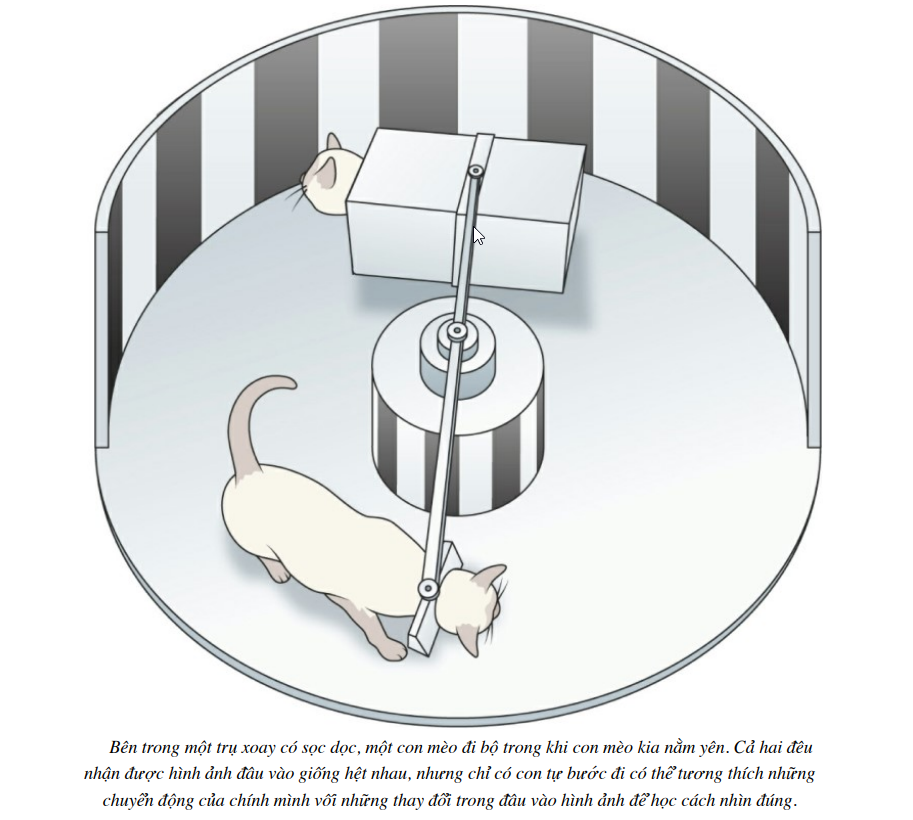
\includegraphics[width=\textwidth]{images/2024-07-30_13h08_25.png}
\tab\tab - TN3: Tiến sĩ Alyssa Brewer tại Đại học California tiến hành thí nghiệm để đo lường khả năng thích nghi của bộ não. 
Cô trang bị cho những người tham gia lăng kính đảo chiều trái-phải của thế giới, các vật ở bên phải xuất hiện bên tay trái của tôi và ngược lại. 
Sau một tuần vật lộn vừa nhìn vừa thử tương tác, cuối cùng những người tham gia thí nghiệm đã làm quen được
Bản đồ không gian của họ về thế giới đã thay đổi. Thêm một thí nghiệm cho thấy việc nhìn không chỉ đơn thuần 
liên quan đến thị giác.\\
\tab\tab - TN4: Robert Luke(Cold Blue Luke) tù nhân khi bị biệt giam trong Hole đến 90 ngày 
(căn phòng dài, rộng tầm 3 mét, tối đen, không âm thanh), đã chia sẻ: "Tôi nhớ rằng mình đi trên 
những chuyến hành trình. Một điều tôi nhớ là tối bay như một con diều. Nó có vẻ thật. Nhưng tất cả 
chỉ ở trong đầu tôi"-> Cho thấy dù bị cắt hết tín hiệu bên ngoài não bộ vẫn tự xây dựng một thế giới.\\
\tab\tab - TN5:\\
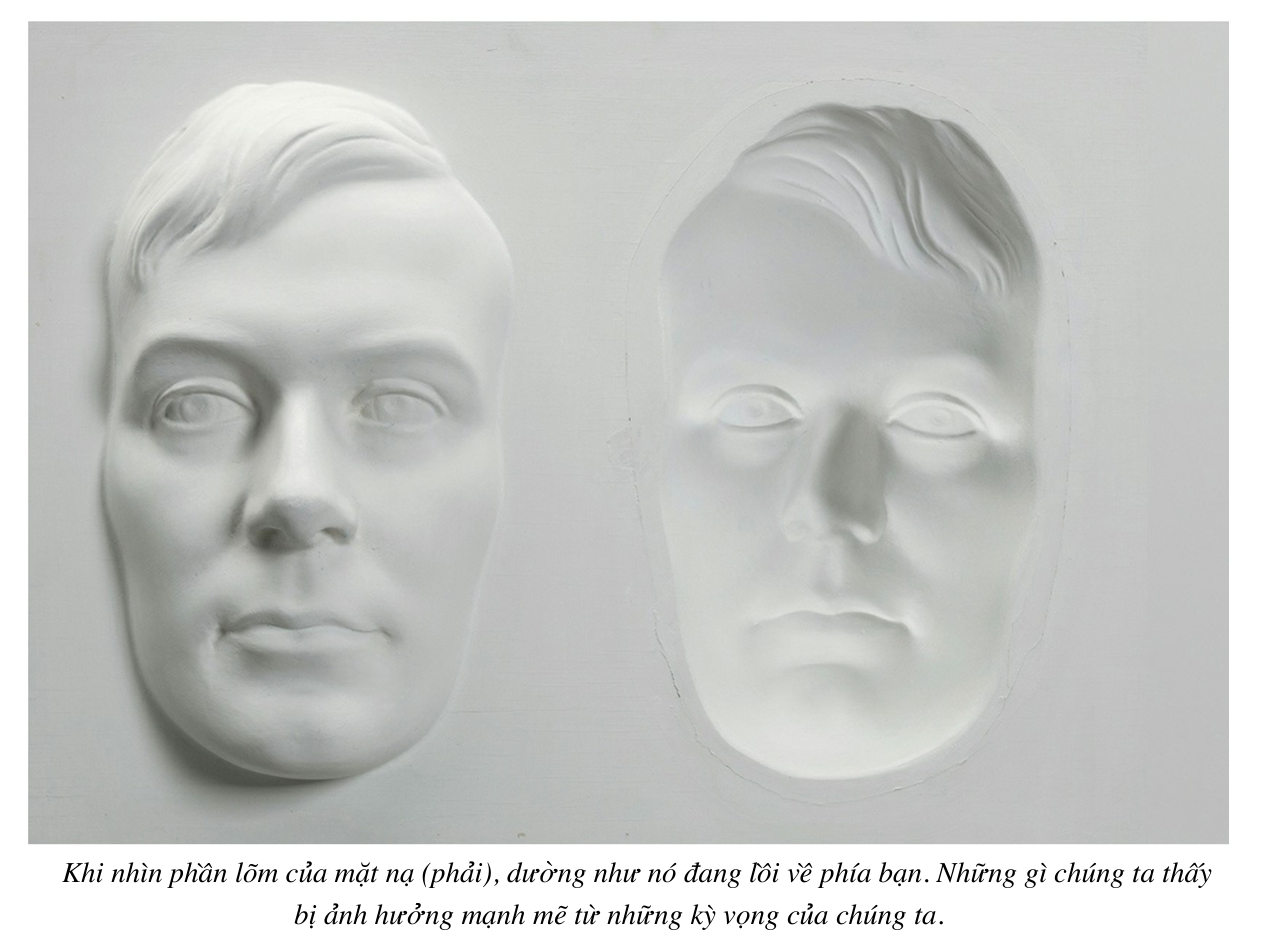
\includegraphics[width=\textwidth]{images/Screenshot 2024-07-30 194516.png}
\tab\tab - TN6: Hannah Bosley. Khi nhìn vào các chữ cái trong
bảng chữ cái, cô ấy có một trải nghiệm nội tâm về màu sắc. Đối với cô, J
màu tím, hoặc T màu đỏ là là hiển nhiên. Hannah không phải là người đầy thi vị hay ẩn dụ - chỉ là cô ấy có một
trải nghiệm cảm giác được gọi là cảm giác thứ phát. -> Thực tại của bạn khác thực tại của tôi.\\
\tab\tab - TN7: nhiều báo cáo của những người gặp nguy hiểm cận kề cái chết cho rằng thời gian
trôi chậm đi khi họ đối mặt với các tình huống này. Để kiểm chứng, tác giả và 21 tình nguyện viên thực hiện 
rơi tự do từ độ cao 45m. Toàn bộ đều đeo 1 màn hình kĩ thuật số vào cổ tay. Những người tham gia 
phải xác định con số được hiển thị trên màn hình. Lần đầu tốc độ bật tắt là chậm, lần sau là nhanh. Với lần chậm
mọi nguời hầu như không gặp khó khăn nhưng lần nhanh thì không ai thấy được cả\\
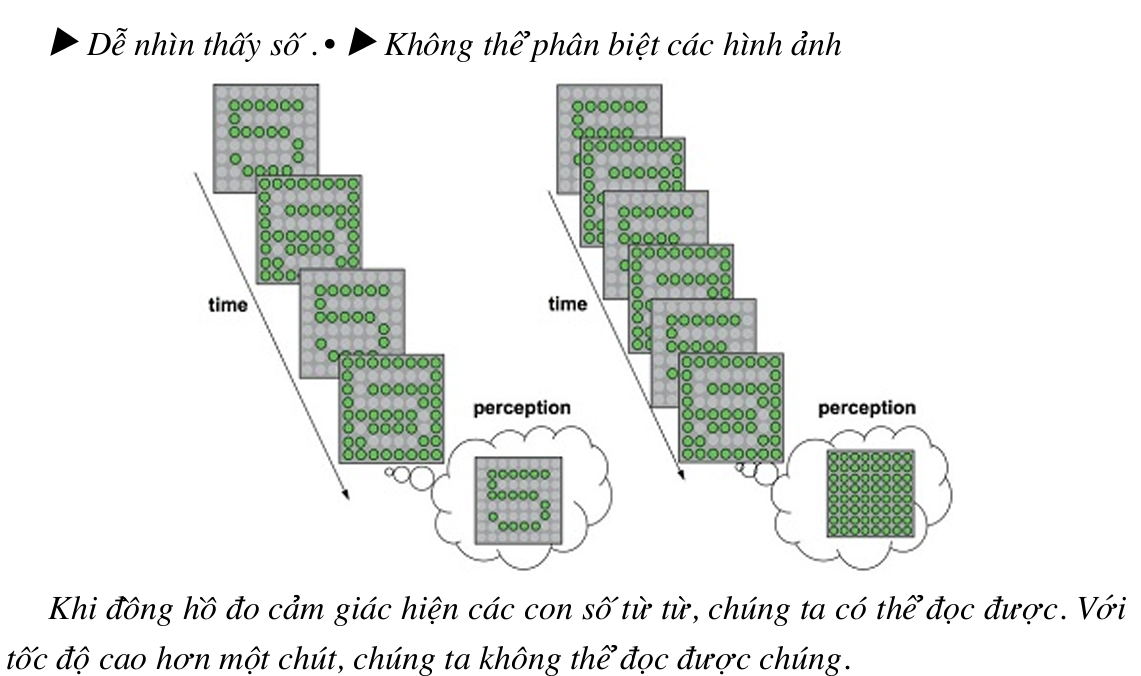
\includegraphics[width=\textwidth]{images/Screenshot 2024-07-30 195407.png}
\tab Như vậy có thể kết luận không phải thời gian trôi chậm đi. Câu trả lời thật ra nằm trong cách kí ức
được lưu trữ.  Trong những tình huống nguy hiểm, một vùng não được gọi là hạch hạnh
nhân (amygdala) được đưa lên trạng thái cao hơn, chỉ huy các nguồn lực
của phần não còn lại và buộc tất cả mọi thứ phải tham gia giải quyết tình
hình hiện tại. Khi hạch hạnh nhân tham gia cuộc chơi, những ký ức được
trải ra với độ chi tiết và phong phú hơn nhiều so với những hoàn cảnh bình
thường; một hệ thống trí nhớ thứ cấp đã được kích hoạt. Rốt cuộc, đó là tác
dụng của trí nhớ: theo dõi các sự kiện quan trọng, để nếu bạn đang ở trong
tình huống tương tự, não bộ sẽ có thêm thông tin cho những nỗ lực tồn tại.
Tác động phụ thú vị nằm ở chỗ: não của bạn không quen với kiểu mật độ
 đó của trí nhớ, vì vậy khi các sự kiện
 được phát lại trong trí nhớ của bạn, thì kết quả là các sự kiện này sẽ chiếm
 nhiều thời gian hơn.\\
 \tab \textbf{Tóm tắt các ý chính}: \\
\tab\tab - Bộ não nhận tín hiệu đầu vào từ các giác quan, tổng hợp rồi từ đó biến đổi các tín hiệu này 
và diễn giải thành hiện thực mà ta đang cảm nhận được.\\
\tab\tab - Do cơ thể sinh học của mỗi người là khác nhau nên thế giới của bạn khác thế giới của tôi.\\
\tab\tab - Thực tế, chúng ta không bao giờ sống ở hiện tại mà đang ở quá khứ\\
\tab\tab - Do giới hạn về mặt sinh học nên thực tại mà ta cảm nhận được chỉ là một
lát cắt của thực tại mà thôi\\


\section{Ai là người điều khiển?}
\section{Chúng ta quyết định như thế nào?}
\section{Tôi có cần bạn?}
\section{Chúng ta sẽ là ai?}



\end{document}